%%%%%%%%%%%%%%%%%%%% author.tex %%%%%%%%%%%%%%%%%%%%%%%%%%%%%%%%%%%
%
% sample root file for your "contribution" to a contributed volume
%
% Use this file as a template for your own input.
%
%%%%%%%%%%%%%%%% Springer %%%%%%%%%%%%%%%%%%%%%%%%%%%%%%%%%%


% RECOMMENDED %%%%%%%%%%%%%%%%%%%%%%%%%%%%%%%%%%%%%%%%%%%%%%%%%%%
\documentclass[graybox]{svmult}
\usepackage{etex}


%\usepackage[english]{babel}
%
\usepackage[utf8]{inputenc}
% choose options for [] as required from the list
% in the Reference Guide

\usepackage{mathptmx}       % selects Times Roman as basic font
\usepackage{helvet}         % selects Helvetica as sans-serif font
\usepackage{courier}        % selects Courier as typewriter font
\usepackage{type1cm}        % activate if the above 3 fonts are
                            % not available on your system
%
\usepackage{makeidx}         % allows index generation
\usepackage[]{graphicx}
%\usepackage[draft]{graphicx}        % standard LaTeX graphics tool
\usepackage[size=small,labelfont=bf]{caption}
                             % when including figure files
\usepackage{multicol}        % used for the two-column index
\usepackage[bottom]{footmisc}% places footnotes at page bottom
\usepackage{pdflscape}
%\usepackage{rotating}
\usepackage{afterpage}
%\usepackage[disable]{todonotes}
\usepackage[colorinlistoftodos,prependcaption]{todonotes}
%\usepackage{todonotes}
\usepackage{subfigure}
\usepackage{setspace}
\usepackage{epstopdf}
\usepackage{flafter} %make sure that the floats are not placed 
%before their definition
\usepackage{times}
\usepackage{bm}
\usepackage{gensymb}  % for degree sign, e.g., temperature
\usepackage{amsmath}
\usepackage{amstext}
\usepackage{array}  %for define the fomats of columns in a table
\usepackage{dcolumn}
\usepackage[T1]{fontenc}
\usepackage{pgfplots}
\usepackage{multirow}
\usepackage{makecell}
\usepackage{tabularx}
\usepackage{adjustbox}
\usepackage{capt-of}
%\usepackage{marginnote}
\usepackage{xargs}   % Use more than one 
%optional parameter in a new commands
%\usepackage{siunitx} %for scientific 
%notation
%%we do this because of a bug of package floatrow
%\let\tmp\newinsert
%\let\newinsert\newbox
%\usepackage{floatrow}
%\let\newinsert\tmp
\usepackage{enumitem} %make items indent when using 
%\begin{enumerate}[(a)]
\usepackage{verbatimbox}  %for \addvbuffer
\usepackage{hyperref}
\usepackage{tikz}
\usepackage{xspace}
%\usepackage{pdfcomment}
%\newcommand*\circled[1]{\tikz[baseline=(char.base)]{
%		\node[shape=circle,draw,inner sep=1pt] (char) {#1};}}
%\newcommand*\circledtwo[1]{\tikz[baseline=(char.base)]{
%		\node[shape=circle,draw,inner sep=0.1pt] (char) {#1};}}
 \newcommand{\maps}{\ensuremath{M_\mathrm{s}}\xspace}
 \newcommand{\mapg}{\ensuremath{M_\mathrm{g}}\xspace}



\usepackage[backend=bibtex,
bibstyle=authoryear, %without indices before names; year after 
%names
%style=authoryear,
citestyle=authoryear,
maxbibnames=20,maxcitenames=2,
firstinits=true,
%terseinits=true, %remove periods after initials of first names
%style=apa, %
%sorting=ydnt, %Sort bibliography by year (descending), name, 
%title
doi=false,isbn=false,url=false,
eprint=false,dashed=false]{biblatex}

%\renewcommand*{\bibfont}{\small} %set the font size of the 
%references
%\renewcommand*{\nameyeardelim}{\addspace} %\remove the comma 
%between author and year citations
%\renewcommand*{\revsdnamepunct}{} %remove commas between last 
%%and first names in bibliography
%\renewcommand{\labelnamepunct}{\addspace} %remove the 
%%punctuation after the year in bibliography
%\renewcommand{\finentrypunct}{} %remove the full stop at the 
%%end of each bibliography entry
\renewcommand*{\revsdnamepunct}{} %remove commas between last 
%and first names in bibliography

%remove "In:" for articles in bibliography
\renewbibmacro{in:}{\ifentrytype{article}{}
	{\printtext{\bibstring{in}\intitlepunct}}} 

\addbibresource{References.bib}



\newcommand{\mypar}[1]{\bigskip\noindent\textbf{#1.}~}

\newcommand{\e}[1]{\times 10^{#1}}
\newcommand{\fig}{Fig.~}
\newcommand{\eq}{Eq.~}
\newcommand{\sect}{Sec.~}
\newcommand{\tab}{Tab.~}

%\newcommand{\myeqref}[1]{Eq.~\ref{#1}}
%\newcommand{\mysectref}[1]{Sec.~\ref{#1}}
%\newcommand{\myfigref}[1]{Fig.~\ref{#1}}
%\newcommand{\mytabref}[1]{Tab.~\ref{#1}}


\newcommand{\dtrm}[2][]{d_{\mathrm{#2}, t\ifthenelse{\equal{#1}{}}{}{_#1}}}


\graphicspath{{figures/}}
\DeclareMathAlphabet{\mathpzc}{OT1}{pzc}{m}{it}

%For the references, the following commands make the titles 
%lowercase while keep the initial letters of journal names 
%uppercase
\DeclareFieldFormat{titlecase}{\MakeSentenceCase*{#1}}
\newbibmacro*{journal}{%
	\iffieldundef{journaltitle}
	{}
	{\printtext[journaltitle]{%
			\printfield[myplain]{journaltitle}%
			\setunit{\subtitlepunct}%
			\printfield[myplain]{journalsubtitle}}}}
\DeclareFieldFormat{myplain}{#1}

%Remove the quotation marks for the titles in the reference
\DeclareFieldFormat[article,inbook,incollection,inproceedings,patent,thesis,unpublished]{citetitle}{#1}
\DeclareFieldFormat[article,inbook,incollection,inproceedings,patent,thesis,unpublished]{title}{#1}
\DeclareNameAlias{author}{last-first}

%%Using \DeclarePairedDelimiter from mathtools, you could define 
%%macros \ceil and \floor, which will scale the delimiters 
%%properly (if starred):
%\usepackage{mathtools}
%\DeclarePairedDelimiter\ceil{\lceil}{\rceil}
%\DeclarePairedDelimiter\floor{\lfloor}{\rfloor}

\pgfplotsset{
	compat=newest,
	xlabel near ticks,
	ylabel near ticks
}


\newcommandx{\marginalcomment}[2][1=]{\todo[linecolor=blue,backgroundcolor=blue!25,bordercolor=blue,#1]{#2}}

\renewcommand{\textfraction}{0.01}
\renewcommand{\topfraction}{0.99}
\renewcommand{\bottomfraction}{0.99}
\renewcommand{\dbltopfraction}{0.99} % fit big float above 
%2-col. text
%\renewcommand\thesection{\arabic{section}}
%\renewcommand\thesubsection{\thesection.\arabic{subsection}}



% see the list of further useful packages
% in the Reference Guide

\makeindex             % used for the subject index
                       % please use the style svind.ist with
                       % your makeindex program

%%%%%%%%%%%%%%%%%%%%%%%%%%%%%%%%%%%%%%%%%%%%%%%%%%%%%%%%%%%%%%%%%%%%%%%%%%%%%%%%%%%%%%%%%

\begin{document}

\title*{Continuous Generalization of Buildings \protect\\ by Growing and 
Merging}
\titlerunning{Continuous Generalization of Buildings}
% Use \titlerunning{Short Title} for an abbreviated version of
% your contribution title if the original one is too long
\author{Dongliang Peng and Guillaume Touya}
% Use \authorrunning{Short Title} for an abbreviated version of
% your contribution title if the original one is too long
\institute{
	Dongliang Peng 
	\at Chair of Computer Science I, University of W\"urzburg, 
	Germany \\
	\email{dongliang.peng@uni-wuerzburg.de}
	\and
	% 
	Guillaume Touya
	\at COGIT, IGN, France \\
	\email{guillaume.touya@ign.fr}
}
%
% Use the package "url.sty" to avoid
% problems with special characters
% used in your e-mail or web address
%
\maketitle

\newcommand{\myabstract}{We propose a method to continuously 
	generalize buildings from a given start scale to a smaller goal scale. 
	%
	If several buildings are close to each other at the start 
	scale, we bridge them by line segments and merge the several buildings into 
	one 
	building.
	For each building, either an original one or a merged one, at the start 
	scale, 
	we generate its target shape at 
	the goal scale by enlarging and simplifying. 
	Then we grow the building to the target shape.
	%
	After finishing the growing, we can take the goal scale as the 
	start scale and repeat the process.
	\newline\indent
	The advantages of our method are as follows. First, the buildings 
	are enlarged continuously. At the same time, they are simplified. 
	Second, we ensure that the distance between any pair of two buildings is 
	always larger than a specified threshold.}





\abstract*{\myabstract}

\abstract{\myabstract}


\keywords{Text, Text}

\section{Introduction}
\label{sec:Introduction}


Digital maps such as Google Maps and OpenStreetMap support zooming by 
displaying maps at different levels. 
This discrete strategy may results in sudden changes, which annoy users.
To provide better zooming experience, continuous generalization aims to 
produce 
a sequence of maps with small incremental changes.
To realize continuous generalization, \textcite{Sester2005_CG} discussed some 
generalization operators for buildings and proposed to morph a building 
between 
its forms at different levels. Morphing has been used to generate intermediate 
representations for two representations at different scales 
\parencite{mnwb-mpstc-08,Peng2013_LSA,Deng2015,Peng2016_Admin}. 
Also aiming at 
realize continuous generalization, \textcite{Chimani2014_Eat} generated a good 
selection sequence for road networks, and 
\textcite{Peng2017_AStar} tried to compute optimal aggregation sequences for 
land-cover areas.

When users zoom out on digital maps, buildings become closer with each other 
and buildings themselves become smaller. 
In order to make sure that the map is 
easily perceived \parencite{Weibel1997}, small building should be eliminated, 
some building should be enlarged, and buildings close to each other should be 
aggregated.
Although algorithms of simplifying buildings have been studied, e.g., 
\textcite{Buchin2011_Simp,haunertwolff2010}, problems become more complicated 
when we have to aggregate buildings simultaneously.
In order to aggregate, we should first group the buildings.





\bigskip

The papers we may review:   
\textcite{vanSmaalen2003, Buchin2016, Chaudhry2008, Stoter2009},

Rules for building simplification; see \textcite{Lee2005}

Straight skeletons for map generalization: 
\textcite{Gold2003,Matuk2006}


An example of enlargement in aggregation: \citetitle{Neun2005}

Using MST to group buildings: \textcite{Zhang2013, 
Cetinkaya2015,Deng2017,Regnauld1996}



\section{Methodology}

\todo[inline]{a brief introduction of our method.}
We name our input map as start map \maps,
and denote the scale of the start maps by $1:S_\mathrm{s}$.
We generate goal map \mapg at scale $1:S_\mathrm{g}$ 
($S_\mathrm{g} > S_\mathrm{s}$) by generalizing \maps. 
We use time $t\in[0,1]$ to define the continuous generalization
process. 
We require that the generalization yields exactly \maps when $t=0$, 
\mapg when $t=1$, 
and that \maps is continuously generalized into \mapg 
when $t$ increases from~$0$ to~$1$.
We define a simple function between scale and time, that is,
$S_t= S_\mathrm{s} + t(S_\mathrm{g}-S_\mathrm{s})$.


\subsection{Grow based on buffering}
\label{sec:Grow}
We grow building based on buffering. 
There are two typical ways of buffering polygons, i.e.,
one with round joins and the other with miter joins (see 
\fig\ref{fig:Buffer_TwoKinds}).
As buildings are usually rectangles, 
we choose the second way because it is 
better at keeping the right angles.
If an angle is acute, however, an excessively long \emph{spike} will be 
produced.
This spike may go across other buildings 
(see \fig\ref{fig:Buffer_MiterLimits}~(a)).
To avoid this kind of interruptions, 
we require that for an angle if a vertex of the 
buffer is more than $\alpha d_\mathrm{G} (\alpha \ge 1)$, 
where $d_\mathrm{G}$ is the growing distance, 
away from the original vertex, 
a \emph{square} joining is applied
(see \fig\ref{fig:Buffer_MiterLimits}~(b)).
To keep right angles of buildings, 
we must have $\alpha \geq \sqrt{2}$. 
We set $\alpha  = 1.5$ so that a square joining is applied when an angle is 
smaller than $83.6 \degree$.

\begin{figure}[tb]
	\centering
	
\includegraphics{Buffer_TwoKinds}
	\caption{Buffering a polygon using different kinds of joins.}
	\label{fig:Buffer_TwoKinds}
\end{figure}

\begin{figure}[tb]
	\centering
	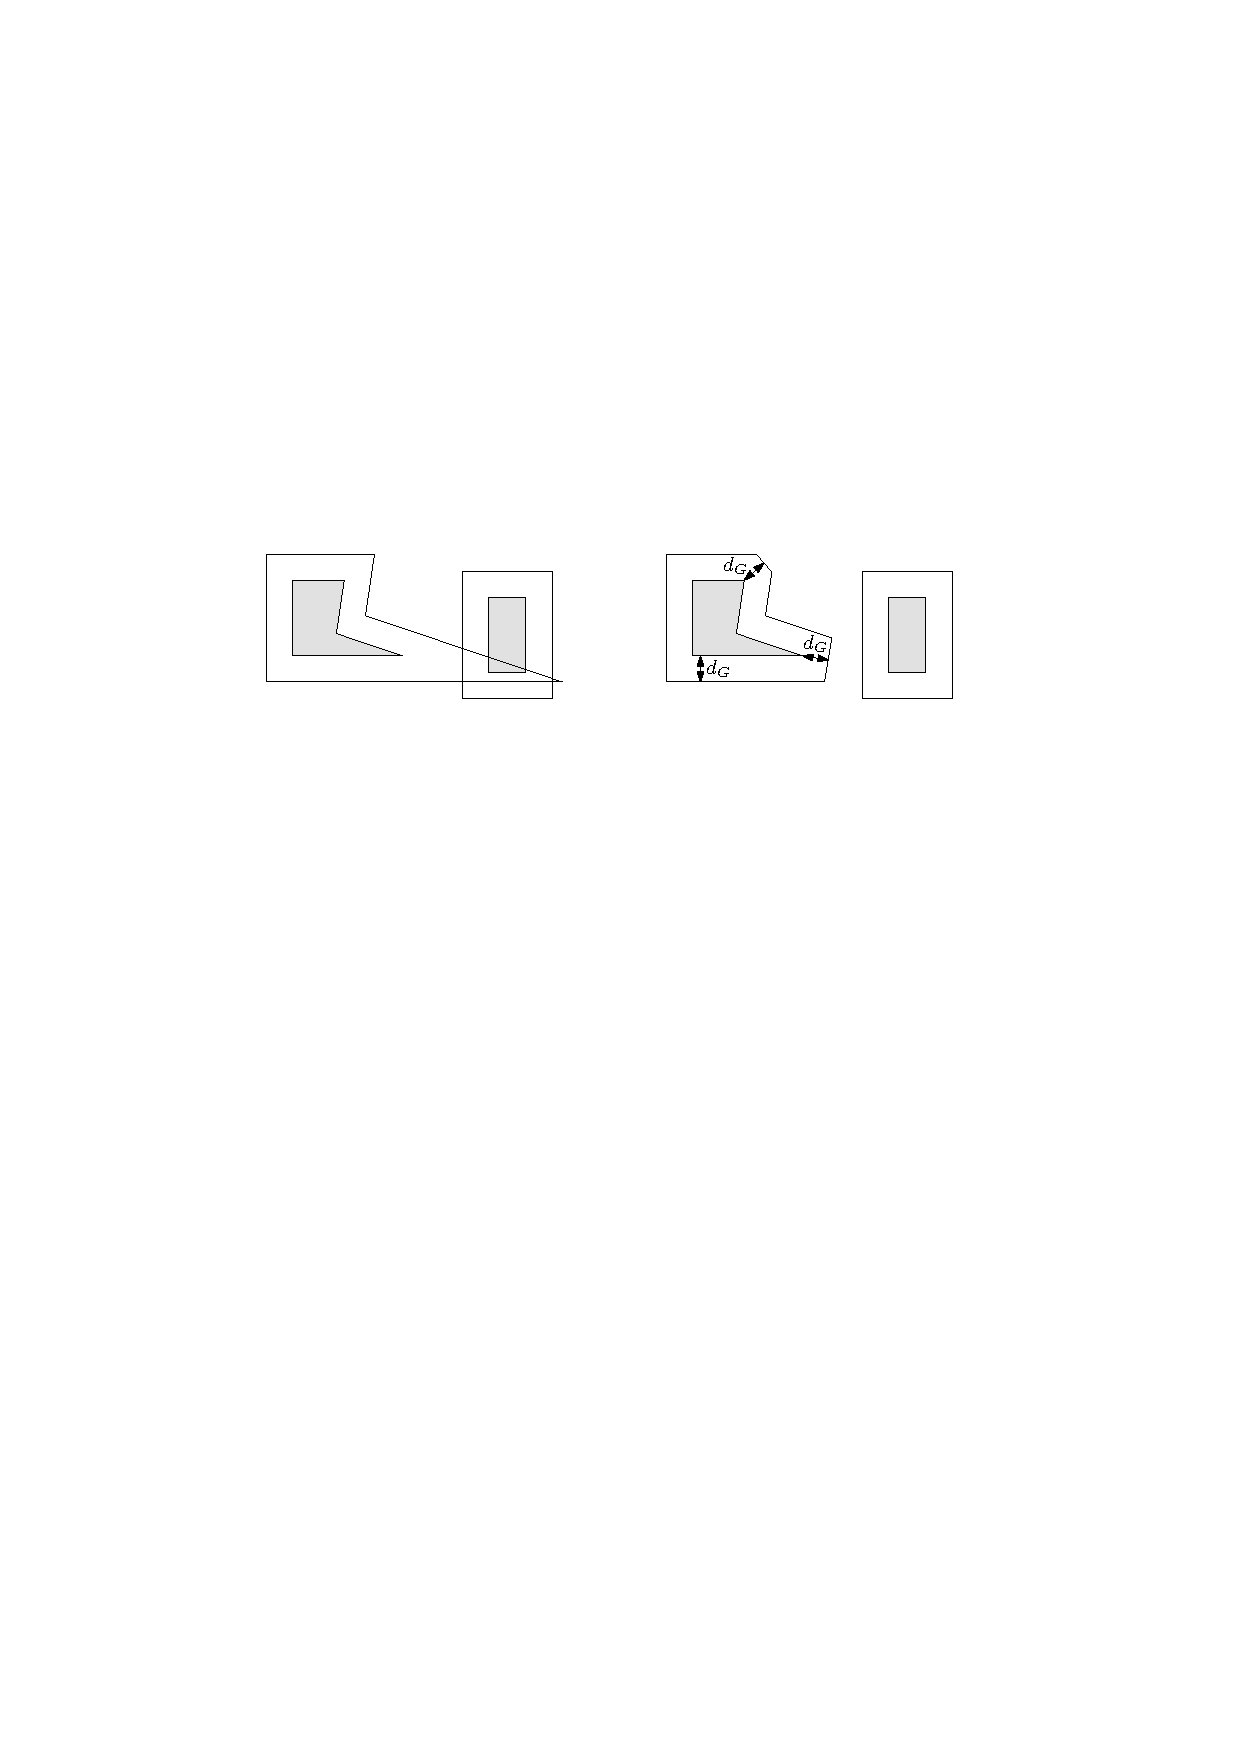
\includegraphics{Buffer_MiterLimits}
	\caption{}
	\label{fig:Buffer_MiterLimits}
\end{figure}


The area of a building on map should be at least $a\,\mathrm{mm}^2$ so that the 
building is large enough to be perceived.
In \sect\ref{sec:Simplify}, we show that we set $a=4$.
Accordingly, a square at the start map should have 
area $a S_\mathrm{s}^2\,\mathrm{mm}^2$ at least, and
a square at the goal map should have 
area $a S_\mathrm{g}^2\,\mathrm{mm}^2$ at least.
The difference of the side lengths is 
$\sqrt{a} (S_\mathrm{g}-S_\mathrm{s})\,\mathrm{mm}$ 
 (see \fig\ref{fig:Growth}).
A square on the start map needs to grow $\frac{1}{2}\sqrt{a} 
(S_\mathrm{g}-S_\mathrm{s})\,\mathrm{mm}$ so that 
it can survive when users zoom out from 
the start map to the goal map.
In order to eliminate small buildings, 
we define our growing distance as
\begin{equation}
\label{eq:d_G}
d_\mathrm{G}=\frac{\lambda}{2}\sqrt{a} (S_\mathrm{g}-S_\mathrm{s})\,\mathrm{mm} 
\quad 0 < \lambda <1,
\end{equation}
where variable $\lambda$ is a growing factor. 
A larger $\lambda$ results in  
fewer buildings to be eliminated, and vice versa.
During our growing, the growth at time $t$ is
\begin{equation}
\label{eq:d_Gt}
\dtrm{G} = t \cdot d_\mathrm{G}.
\end{equation}

\begin{figure}[tb]
	\centering
	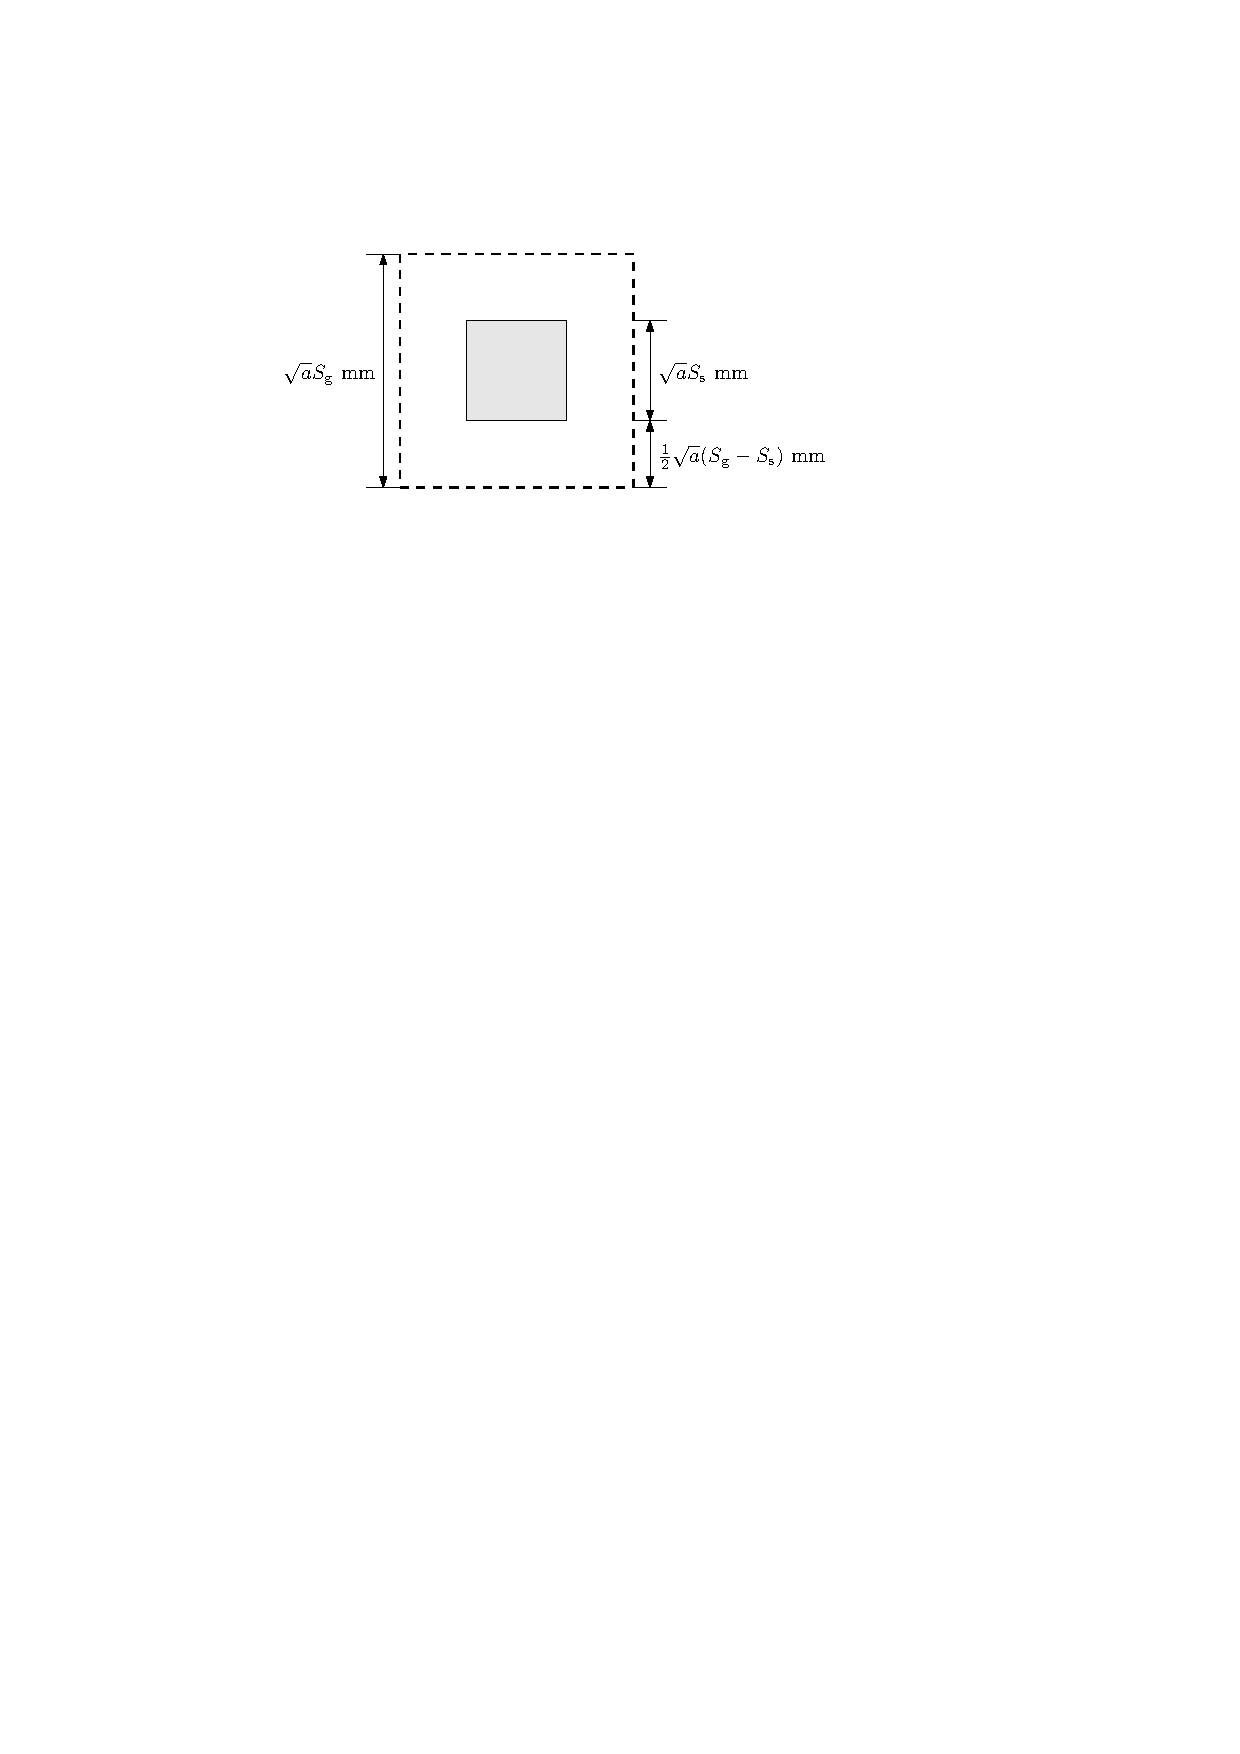
\includegraphics{Growth}
	\caption{Growth.}
	\label{fig:Growth}
\end{figure}


\subsection{Merge close buildings by introducing bridges}
The distance between two buildings should be larger than a threshold
\parencite{Regnauld2001,Li2004}.
Following \textcite{Basaraner2008,Stoter2009}, 
we set the separation threshold $\epsilon= 0.2\,\mathrm{mm}$ for target map. 
The separation threshold at time $t$ is
\begin{equation}
\label{eq:d_epsilont}
d_{\epsilon, t} = \epsilon \cdot S_t.
\end{equation}

If two buildings become too close to each other during growing, 
we merge them by introducing a bridge connecting the nearest points 
(see \fig\ref{fig:GrowAndBridge}).
No matter a bridge appear earlier or later, 
it has width $2\dtrm{G}$ at time $t$.
This setting guarantees that no bridge is thin when $t=1$.
For example, the two bridges in \fig\ref{fig:GrowAndBridge} at time $t=1$ have 
the same widths.
This setting is achieved by following.
We detect nearest points for each pair of buildings at time $t=0$ so that 
we know where we should add bridges. 
We grow the bridges together with the buildings,
but we do not show the bridges until the two buildings are close enough. 
\todo[inline]{actually larger than $d_{\epsilon, t}$.}


\begin{figure}[tb]
	\centering
	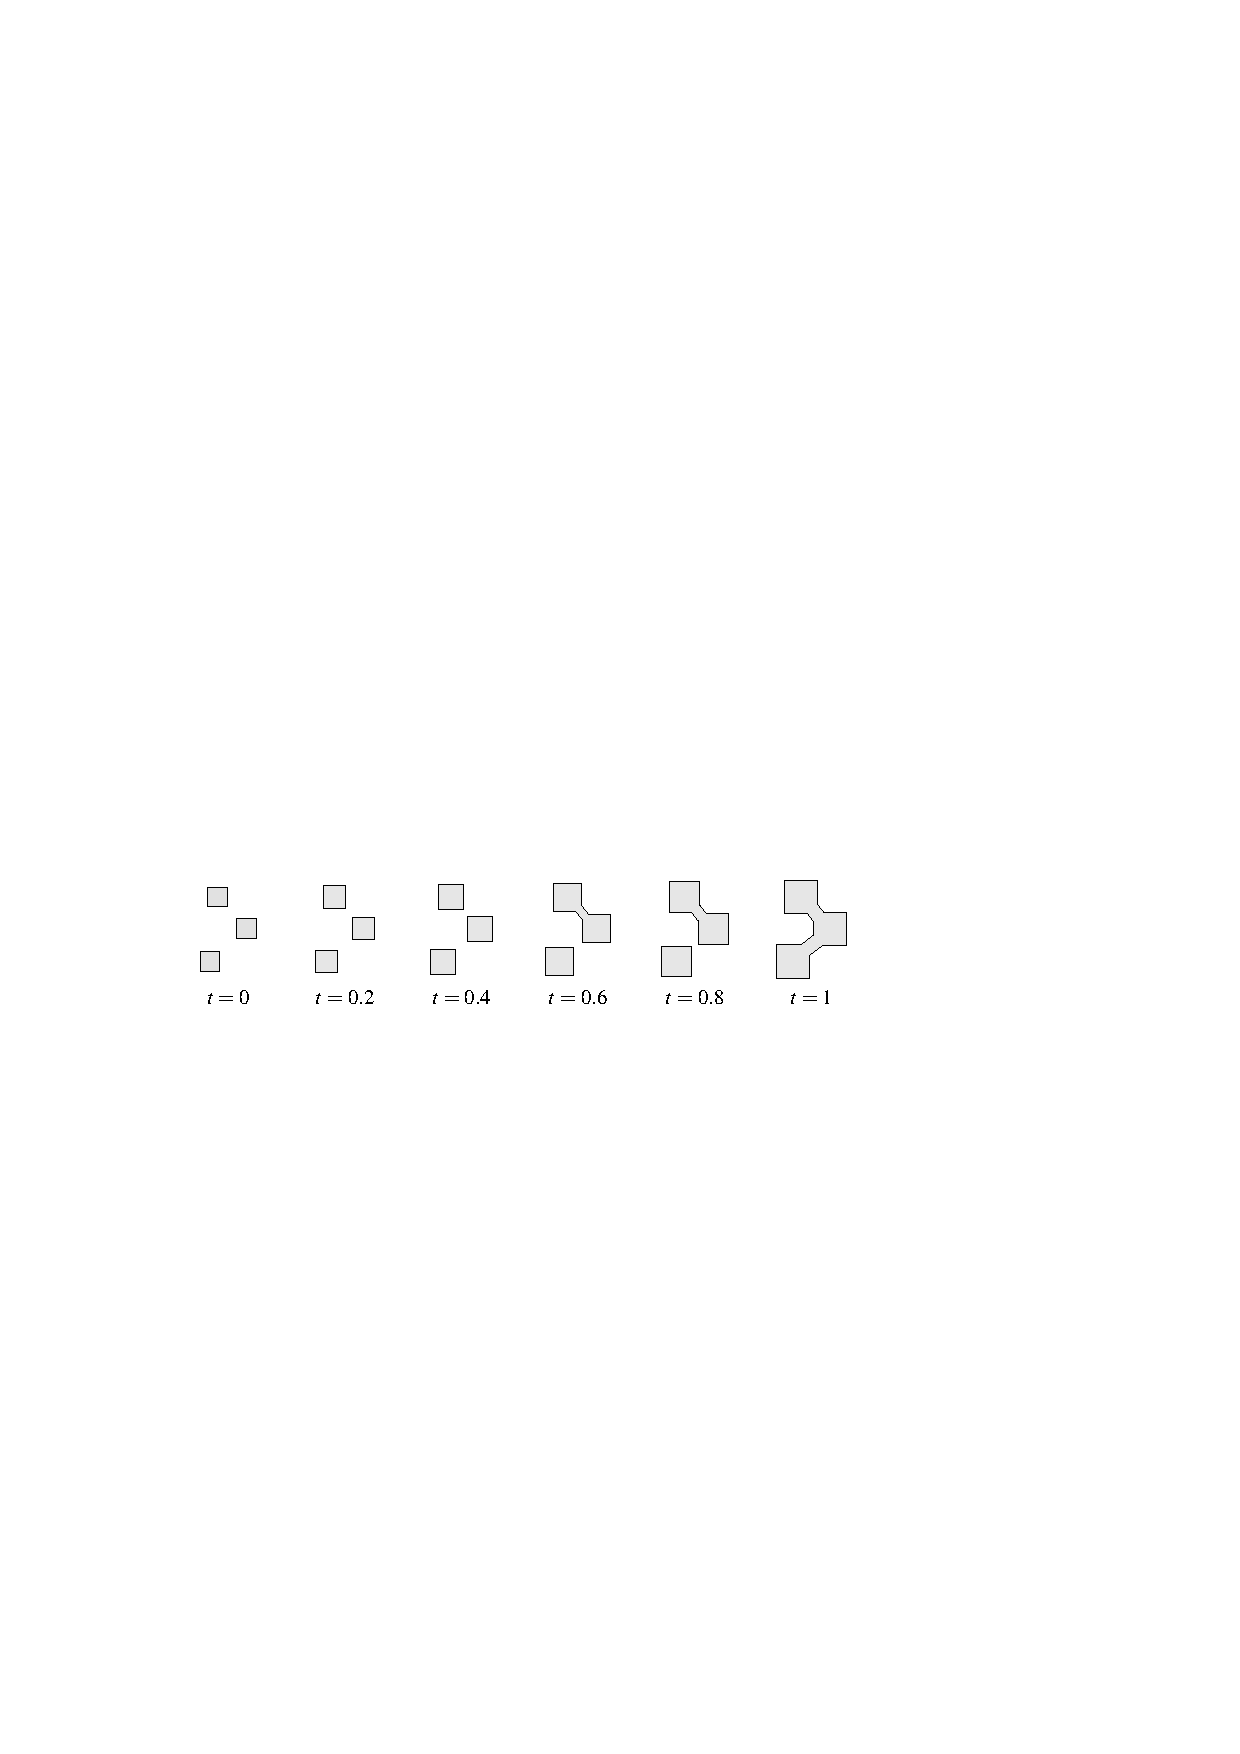
\includegraphics{GrowAndBridge}
	\caption{Merge buildings by introducing bridges when the buildings become 
	too close.
		Although the bridges appear at different time, 
		their widths are the same (see the figure with $t=1$).}
	\label{fig:GrowAndBridge}
\end{figure}


\subsection{Simplify grown buildings}
\label{sec:Simplify}
We use a buffering-based method, 
similar to \textcite{Damen2008,Meijers2016}, 
to simplify our grown buildings. 
We first dilate the grown buildings to remove 
pits, and then erode the results to remove spikes
(see \fig\ref{fig:RemovePitAndSpike}).

\begin{figure}[tb]
	\centering
	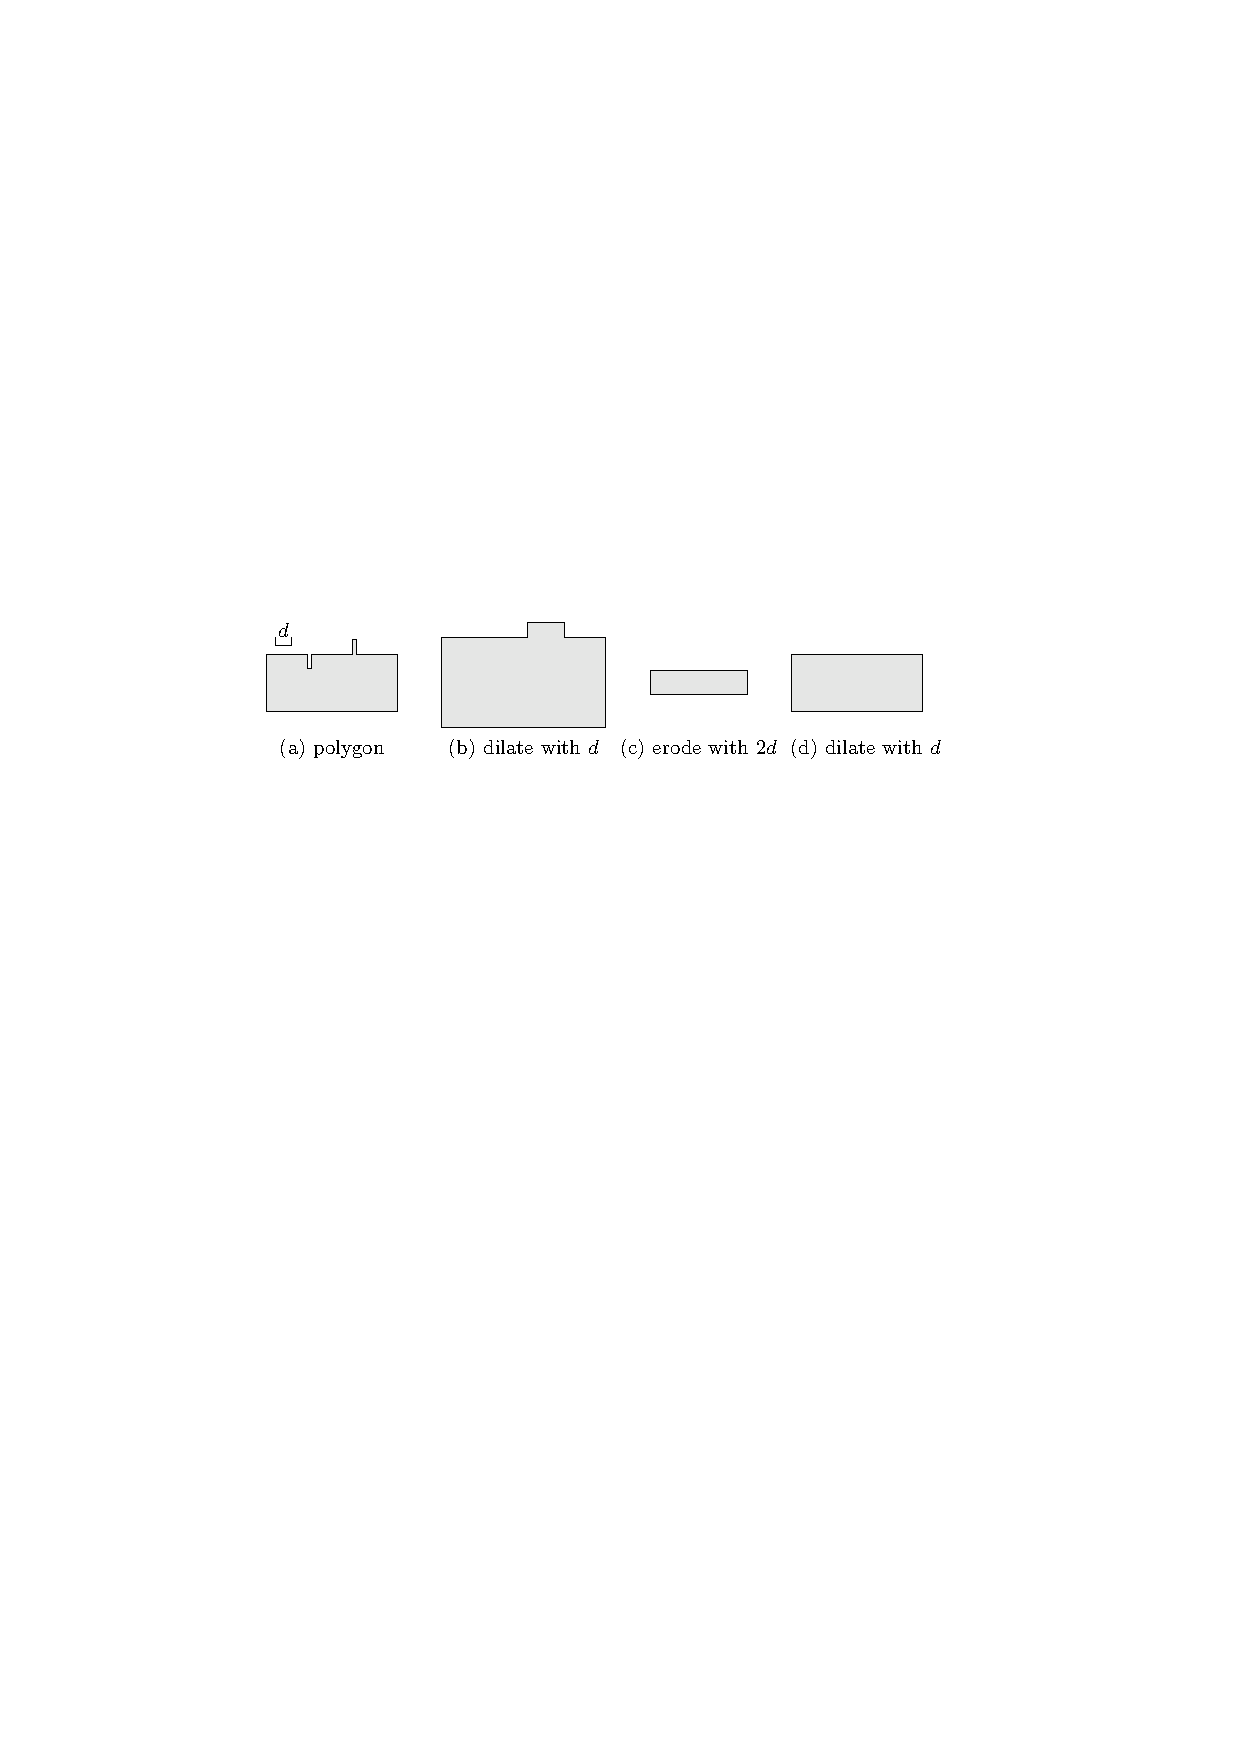
\includegraphics[draft=true]{RemovePitAndSpike}
	\caption{Remove a pit by dilating and then remove a spike by eroding.
		(a) a polygon with a pit and a spike;
		(b) dilate the polygon in (a) with distance $d$ to remove the pit;
		(c) erode the polygon in (b) with distance $2d$ to remove the spike;
		(d) dilate the polygon in (c) with distance $d$ so that the result has 
		the same size as the polygon in (a).
	}
	\label{fig:RemovePitAndSpike}
\end{figure}

At time $t$, we grow buildings with distance $\dtrm{G}$,
dilate with distance $\dtrm{D} (\dtrm{D}>0)$,
erode with distance $\dtrm{D}+\dtrm{E} (\dtrm{E}>0)$,
and dilate back with distance $\dtrm{E}$.
A problem we may have is that we may break a building by eroding.
The reason is that 
some parts of a building may be increased (by growing and dilating) 
with distance $\dtrm{G}+\dtrm{D}$, 
but be decreased (by eroding) as much as $\alpha (\dtrm{D}+\dtrm{E})$.
If  $\dtrm{G}+\dtrm{D} < \alpha (\dtrm{D}+\dtrm{E})$ 
and a building is not thick enough, 
the building may be broken into several parts
(see \fig\ref{fig:ErosionBreak}).
In order to avoid this problem, we require that
\[
\dtrm{G} + \dtrm{D} \ge \alpha (\dtrm{D}+\dtrm{E}),
\]
which means
\begin{equation}
\label{eq:d_Dt}
\dtrm{D} \le \frac{\dtrm{G}-\dtrm{E}}{\alpha - 1}.
\end{equation}

\begin{figure}[tb]
	\centering
	
\includegraphics[draft=false]{ErosionBreak}
	\caption{Dilate the gray polygon, then erode the dilated polygon.
		(a) Dilate and erode with distance $d_1$.
		(b) Dilate and erode with distance $d_2$, where $d_2>d_1$.
		In (a) the result of dilation and erosion is the same as the original 
		polygon, while in (b) the result consists of two parts.
	}
	\label{fig:ErosionBreak}
\end{figure}

We would like to use $\dtrm{E}=\frac{l}{2} \cdot S_t$
(see \eq\ref{eq:d_epsilont}) so that
any pits and spikes narrower than $l$ will be removed. 
We set $l=0.3\,\mathrm{mm}$, which was used as a length threshold by 
\textcite{Regnauld2001,Li2004,Basaraner2008}.
According to \eq\ref{eq:d_Gt}, $\dtrm{G}$ can be arbitrarily small 
when $t$ is small, 
but $d_{\epsilon, t}$ is at least $\frac{l}{2} S_\mathrm{s}$. 
In this case, $\dtrm{G}-\dtrm{E} \le 0$ when $t$ is small, 
which violates \eq\ref{eq:d_Dt}, where $\dtrm{D}>0$.
As a compromise, we use
\begin{equation}
\label{eq:d_Et}
\dtrm{E} =t \cdot \frac{l}{2} S_\mathrm{g}.
\end{equation}
Still, we should make sure that $\dtrm{G}-\dtrm{E} > 0$, which means
$t \cdot \frac{\lambda}{2}\sqrt{a} (S_\mathrm{g}-S_\mathrm{s})-
t \cdot \frac{l}{2} S_\mathrm{g} >0$.
As a result, we should make sure that
\begin{equation}
\label{eq:S_g}
S_\mathrm{g} > \frac{\lambda\sqrt{a}}{\lambda\sqrt{a}-l} S_s.
\end{equation}

We wish to remove ``bays'' which have ``widths'' less than $2\sqrt{a_h/\pi}$.
\todo{why? more details}
Usually, our $\dtrm{D}$ is not large enough to do so.
We use the upper bound in \eq\ref{eq:d_Dt}, that is,
\[
\dtrm{D} = \frac{\dtrm{G}-\dtrm{E}}{\alpha - 1}.
\]

After carrying out the buffering-based methods, 
we simplify the grown buildings using Imai--Iri algorithm 
\parencite{ImaiIri1988}.
This algorithm first finds all the valid shortcuts of a polyline.
A shortcut is valid for a segment 
if the distance between the segment and the shortcut is at most a specified 
value
(see \fig\ref{fig:ImaiIri_Shortcut}).
We set the value also as $l$. 
Second, the algorithm finds a sequence of valid shortcuts, from the beginning 
of a polyline to the end, using breadth-first search.
The sequence of valid shortcuts is an approximation of the polyline, 
and has the least number of line segments.

\begin{figure}[tb]
	\centering
	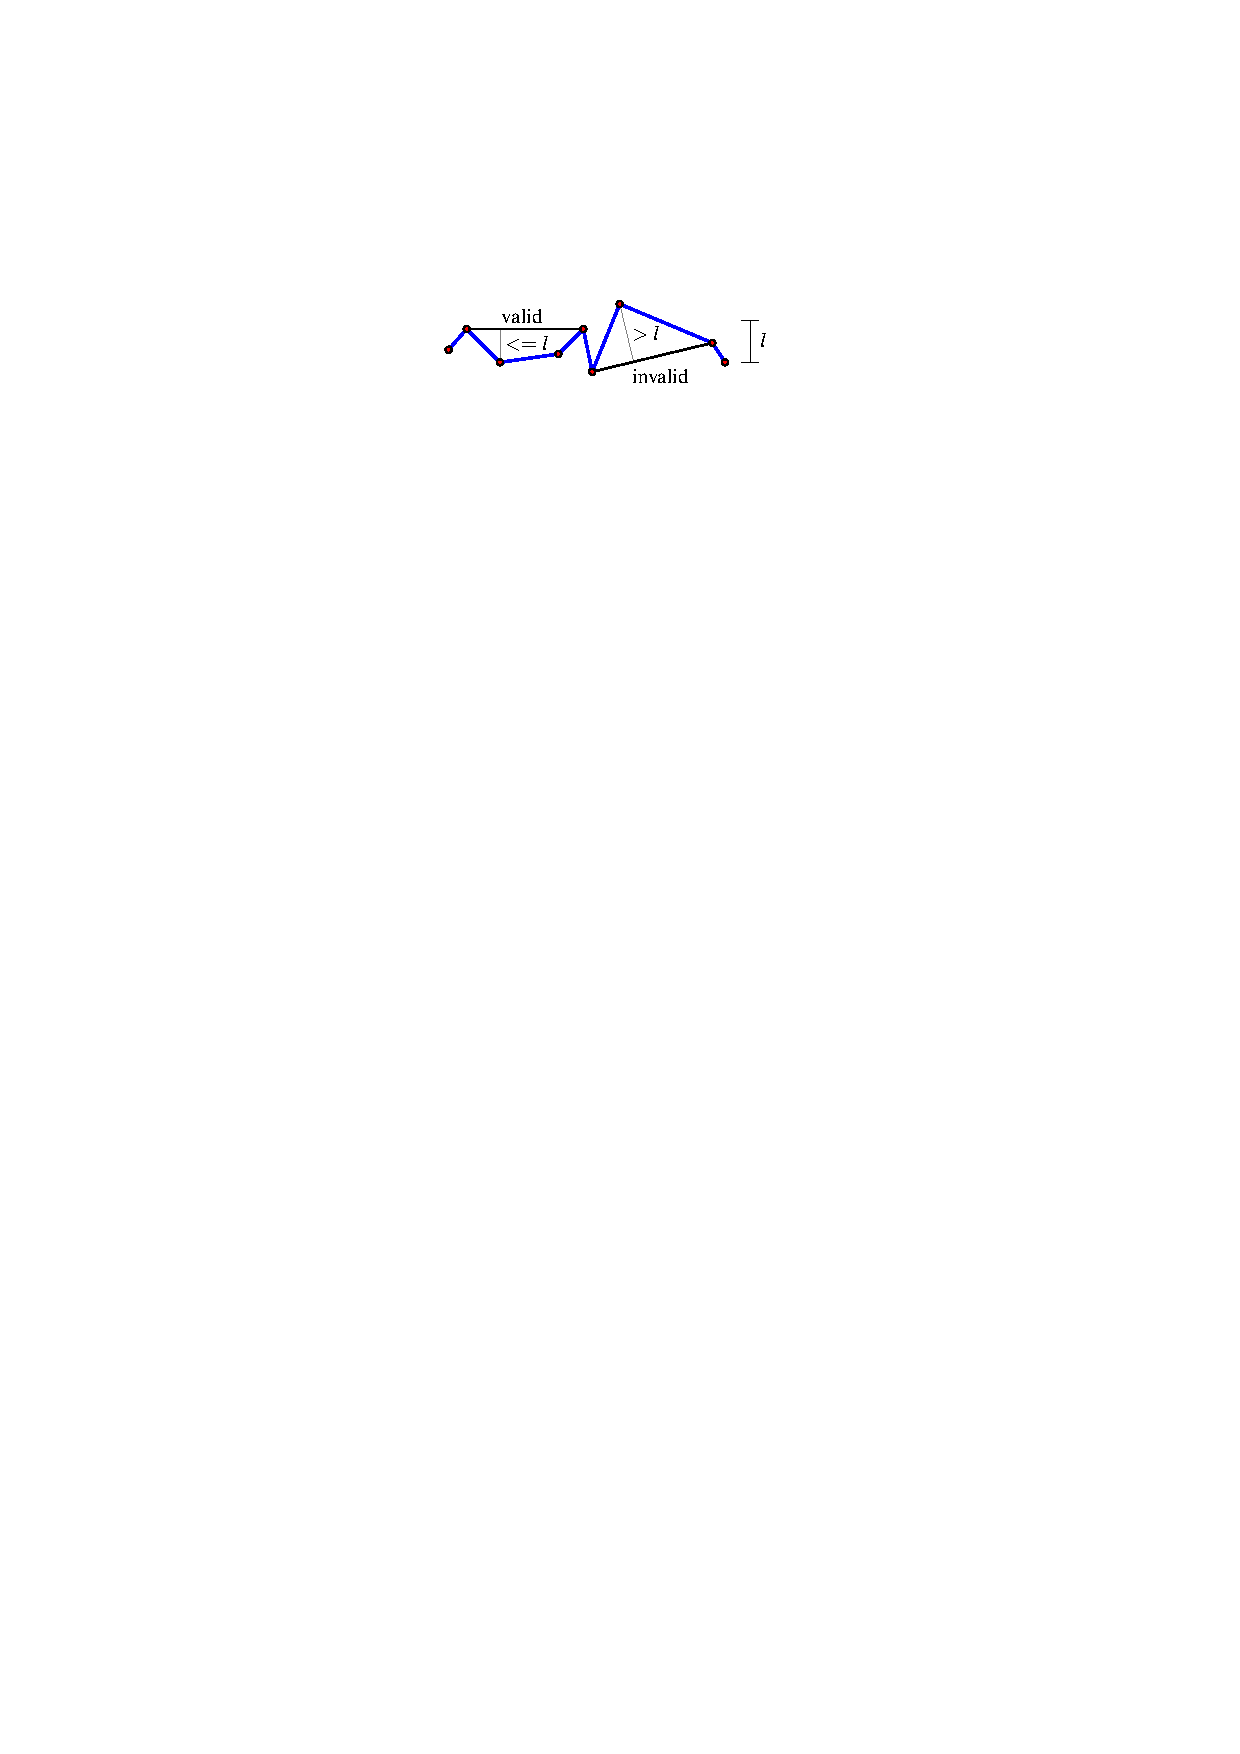
\includegraphics[draft=false]{ImaiIri_Shortcut}
	\caption{Valid and invalid shortcuts for Imai--Iri algorithm.}
	\label{fig:ImaiIri_Shortcut}
\end{figure}

\todo[inline]{more details in the below paragraph?}
We add two more constraints for a shortcut to be valid. 
First, a shortcut must be completely inside the grown building.
If a shortcut is outside,
we are not able to arrive at the shortcut by growing.
Second, a shortcut is not allowed to intersect the 
boundary of the original building.
If we allow this intersection, 
we need to shrink the building instead of growing. 
Of course, we do not want to shrink.

We tried simplifying using Douglas--Peucker algorithm \parencite{Douglas1973}, 
but we hoped to remove more points. We found that the Imai--Iri 
algorithm fit our needs better. 






\subsection{Unite buildings of the immediate previous step}
\label{sec:Unite}

As shown in \eq\ref{eq:d_Et}, $\dtrm{E}$ increases along with time $t$.
We illustrated in \fig\ref{fig:ErosionBreak} that 
a larger $\dtrm{E}$ may result in the shrinking of a building.

$\dtrm[1]{G} + \dtrm[1]{D}$

\begin{figure}[tb]
	\centering
	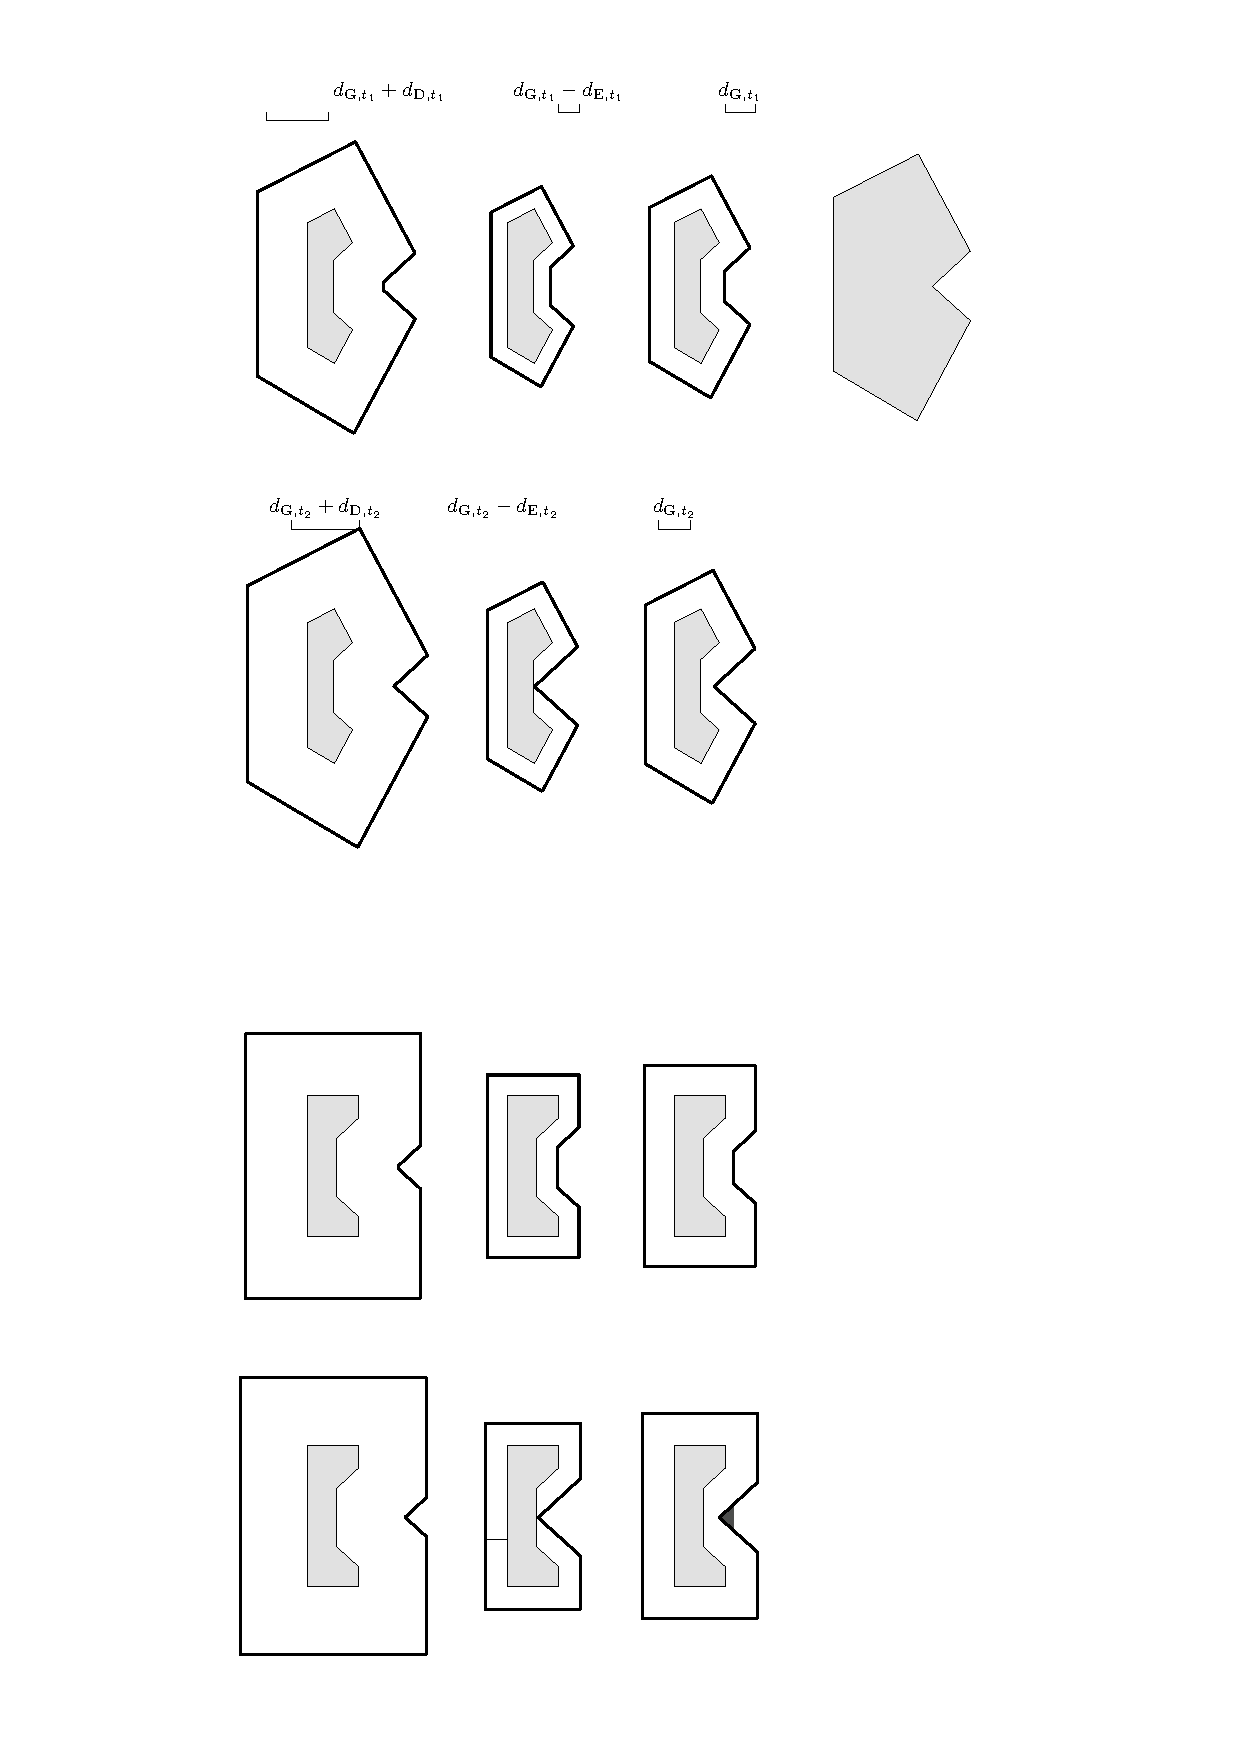
\includegraphics[draft=false]{Shrink_Erosion}
	\caption{.
	}
	\label{fig:Shrink_Erosion}
\end{figure}


As we simplify buildings after growing, 
some parts of the buildings may shrink 
comparing to themselves at the immediate previous steps.
To avoid this shrink, we unite a building with itself at the immediate previous 
step so that the 
united building is always larger than both of the united parts.


\subsection{Eliminate small buildings}
\label{sec:Eliminate}
We eliminate a building if the area of this building is smaller than a 
threshold.
For a group of buildings, we consider the area sum of all the buildings.


\subsection{Group buildings based on buffering}
\label{sec:Grouping}
We group buildings based on the buffers of the buildings. 
We buffer each building with distance $d_G + \frac{d_\epsilon}{2}$, 
where distance $d_G$ is the growing amount of each building. 
Parameter $d_\epsilon$ is the least distance allowed between two buildings.
We grow an additional $\frac{d_\epsilon}{2}$ so that if two buffers overlap, 
the corresponding two buildings will become too close during our growing step.
The two buildings are identified as in the same group.

We merge the buffers which overlap each others so that we have some large units.
Now we iteratively remove small ``bays''.
Each iteration consists of three steps, i.e., 
buffering with distance $r_H$, buffering with distance $-r_H$, and
merging overlapping units.
The iterative process stops when the number of units do not decrease anymore.

All the buildings overlapping with the same unit belong to the same group.



\subsection{Enlarging and merging buildings for goal map}
For each pair of buildings in the same group, 
we find the smallest distance between them.
We connect the buildings by adding an edge from the nearest points.
We find a minimum spanning tree of the buildings using Prim's algorithm 
\parencite{Prim1957}.
We enlarge and merge buildings as the way we do in \sect\ref{sec:Grouping}.






\subsection{Parameters for growing and simplifying}




If we insist on that we should observe 
the growing, say, $x \% (0<x<100)$ of the time at least, then we should make 
sure that
\begin{equation}
\label{eq:a_limit}
\frac{d_\mathrm{G}}{d_\mathrm{G}+d_\epsilon} \ge x \%.
\end{equation}
Using $d_\mathrm{G}$ and $d_\epsilon$ from Eqs.~\ref{eq:d_G} 
and~\ref{eq:d_epsilon}, we transform Eq.~\ref{eq:a_limit} to
\begin{equation}
a \ge \Big(\frac{2 \epsilon S_g x}{\lambda (100-x) (S_g-S_s)}\Big)^2
\end{equation}
We also require 
that $S_g \ge 2 S_s$, which means $S_s \le \frac{1}{2} S_g$.
On one hand, we should have a large $x$ so that we will see the 
growing most of the time.
On the other hand, we wish to keep bridges short as bridges are intrusions to 
our map, which means we should have a small $x$ and a large $\lambda$ so that 
we will have a small 
$a$ (according to Eq.~\ref{eq:a_limit}), a small $d_\mathrm{G}$ (according to 
Eq.~\ref{eq:d_G}), and finally a small $l_b$ (according to 
Eq.~\ref{eq:BridgeLength}). Also we should have a small $x$ and a large 
$\lambda$ as our $a$ is already much larger than $0.16\,\mathrm{mm}^2$ on 
map, which is the area limit used by \textcite{Stoter2009}. As a result, we 
set 
$\lambda=0.8$ and $x=\frac{2}{3} \cdot 100$.
Using these setting, we have
\begin{equation}
a \ge 4.
\end{equation}
according to Eq.~\ref{eq:a_limit}.




Therefore, we may grow up to distance 
\[
D_\mathrm{G} = d_\mathrm{G} + d_\epsilon.
\]
Fig.~\ref{fig:ExtraGrowth} shows such an enlargement and simplification, 
where  
variable $d_\mathrm{e} (\le d_\epsilon)$ is the extra growing distance.


\textcite{Chaudhry2008} thought that a hole of a settlement should be at least 
$0.5\,\mathrm{km}^2$ for a map at scale $1:250{,}000$, 
which means that the hole is at least $8\,\mathrm{mm}^2$ on map. 
Following their setting, we shrink a hole and 
eliminate the hole once its size is smaller than $8\,\mathrm{mm}^2$ on map.







%
%A hole has area less than $\pi D_\mathrm{G}^2$ can be filled by growing. 
%A hole has area 
%slightly more than $\pi D_\mathrm{G}^2$ will become a very small hole after 
%growing with 
%distance $D_\mathrm{G}$. In order to avoid small holes, we do not fill a hole 
%unless the 
%area of the hole on the start map is smaller than $\pi D_\mathrm{G}^2$. Note 
%that we do 
%not fill a hole even if the hole has a large area because a large hole may be 
%split into several small holes by filling. 
%Although our intermediate results may violate the rule that a hole should be 
%at 
%least some size, we try to avoid the violation for a map at a goal scale.
%\textcite{Chaudhry2008} thought that a hole of a settlement should be at 
%least 
%$0.5$ km$^2$ for a map at scale $1:250{,}000$, which means that the hole is 
%at 
%least $8\,\mathrm{mm}^2$ on the map. Following their setting, we wish to have 
%$\pi 
%D_\mathrm{G}^2 \ge 8 S_g^2$.
%
%
%Now we discuss how to set the parameters according to our requirements. 
%First, 
%we wish to increase $d_\mathrm{G}/d_\epsilon$. Most part of a building will 
%grow $d_\mathrm{G}$. Only a small part will continue growing after the 
%building 
%has grown $d_\mathrm{G}$. To ensure that we can see the growing most of the 
%time, we want to have a large $d_\mathrm{G}/d_\epsilon$.
%
%
%
%
%
%We cannot fulfill all the requirements. 

\begin{figure}[tb]
	\centering
	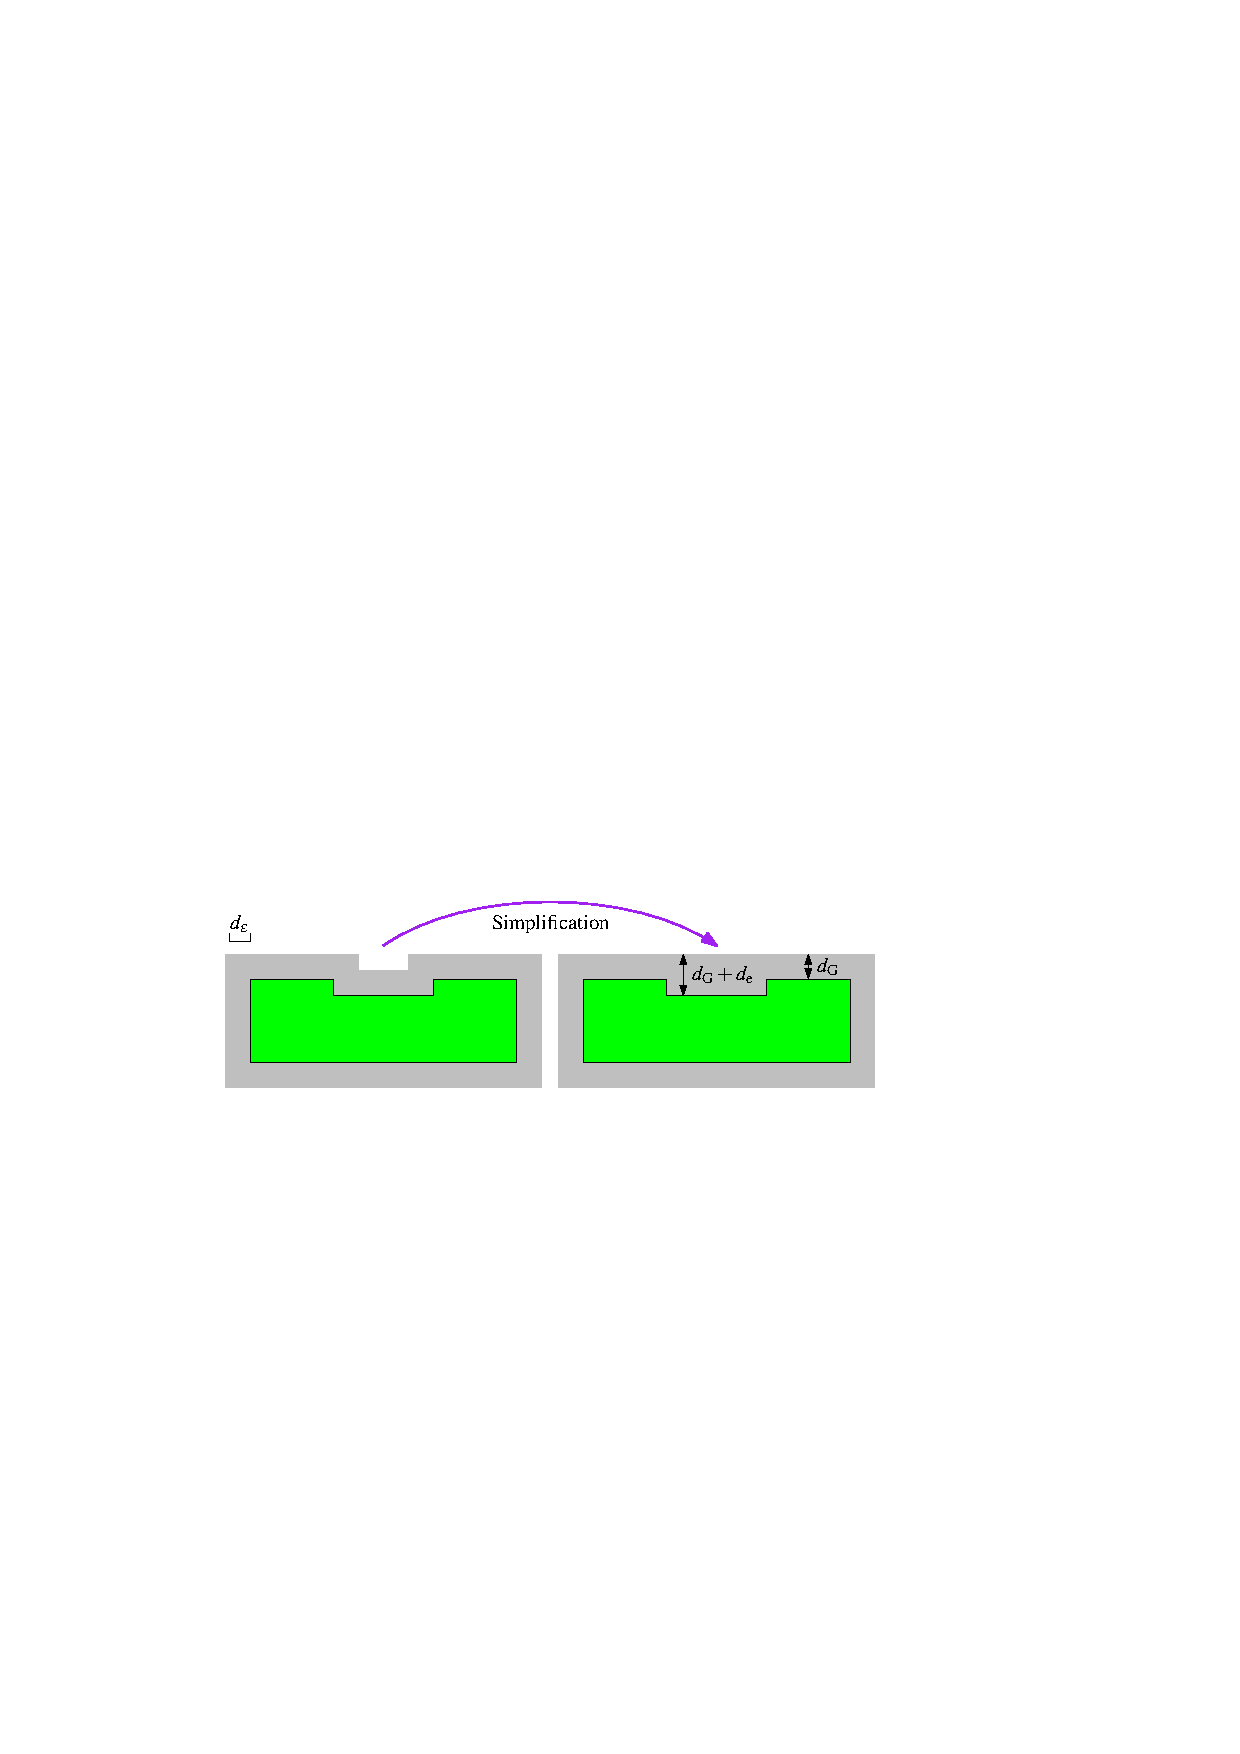
\includegraphics{ExtraGrowth}
	\caption{In the left figure, the green polygon represents a building, and 
	the gray polygon is the enlargement of the building. In the right 
	figure, the gray polygon has been simplified to a rectangle. In order to 
	fill the rectangle, most parts of the (green) building needs to grow with
	distance $d_\mathrm{G}$, but the pit needs to grow with $d_G + 
	d_\mathrm{e}$, 
	where $d_\mathrm{e}$ is the extra growing distance.}
	\label{fig:ExtraGrowth}
\end{figure}


\begin{figure}[tb]
	\centering
	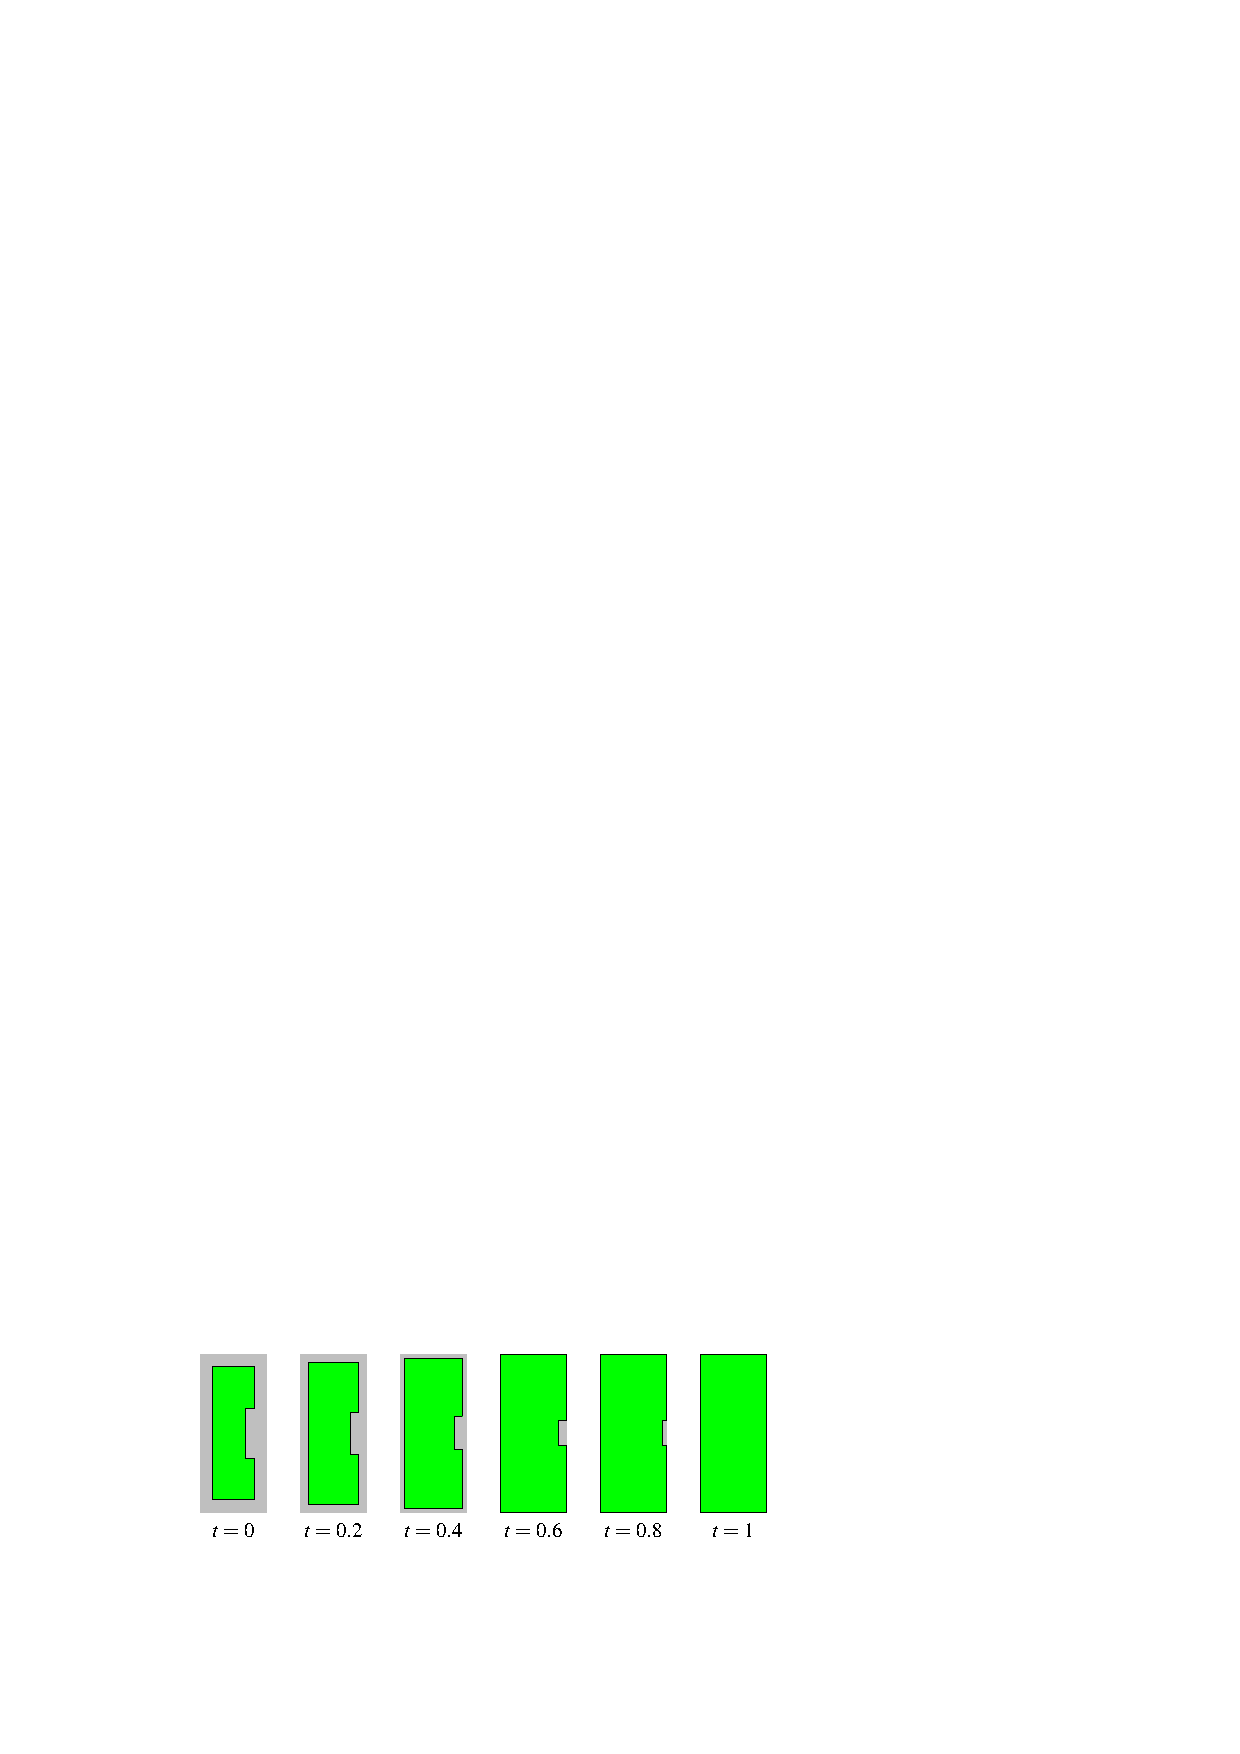
\includegraphics{GrowingExample}
	\caption{GrowingExample.}
	\label{fig:GrowingExample}
\end{figure}

\subsection{Running time analysis}
Although a version with a 
lower running time exists \parencite[see][]{Chan1992}, we implemented the basic 
version.


\section{Case Study}
\label{sec:CaseStudy}
We have implemented our method based on
C\# (Microsoft Visual Studio 2015) and ArcObjects SDK 10.4.1.
The buffer function and clip function are from library \emph{Clipper} 
of \textcite{Johnson2014}.
An evaluation of Clipper can be found in \textcite{Palfrader2015}.
We ran our case study under 64-bit 
Windows 7 on a 3.3 GHz dual core CPU with 8 GB RAM.
We measured processing time by the built-in C\# class 
\emph{Stopwatch}.
We tested our method on a dataset from French Mapping Agency (IGN).
The dataset represents four towns (communes in French), i.e., Aussevielle, 
Denguin,  Poey-de-Lescar, and Siros, in the 
Pyr\'en\'ees-Atlantiques department, south-western France.
The scale of the dataset is $1:15{,}000$.
There are $2{,}590$ buildings (see \fig\ref{fig:Data}), 
which has $19{,}255$ edges in total.
Our goal scale is $1:50{,}000$.


\begin{figure}[tb]
	\centering
	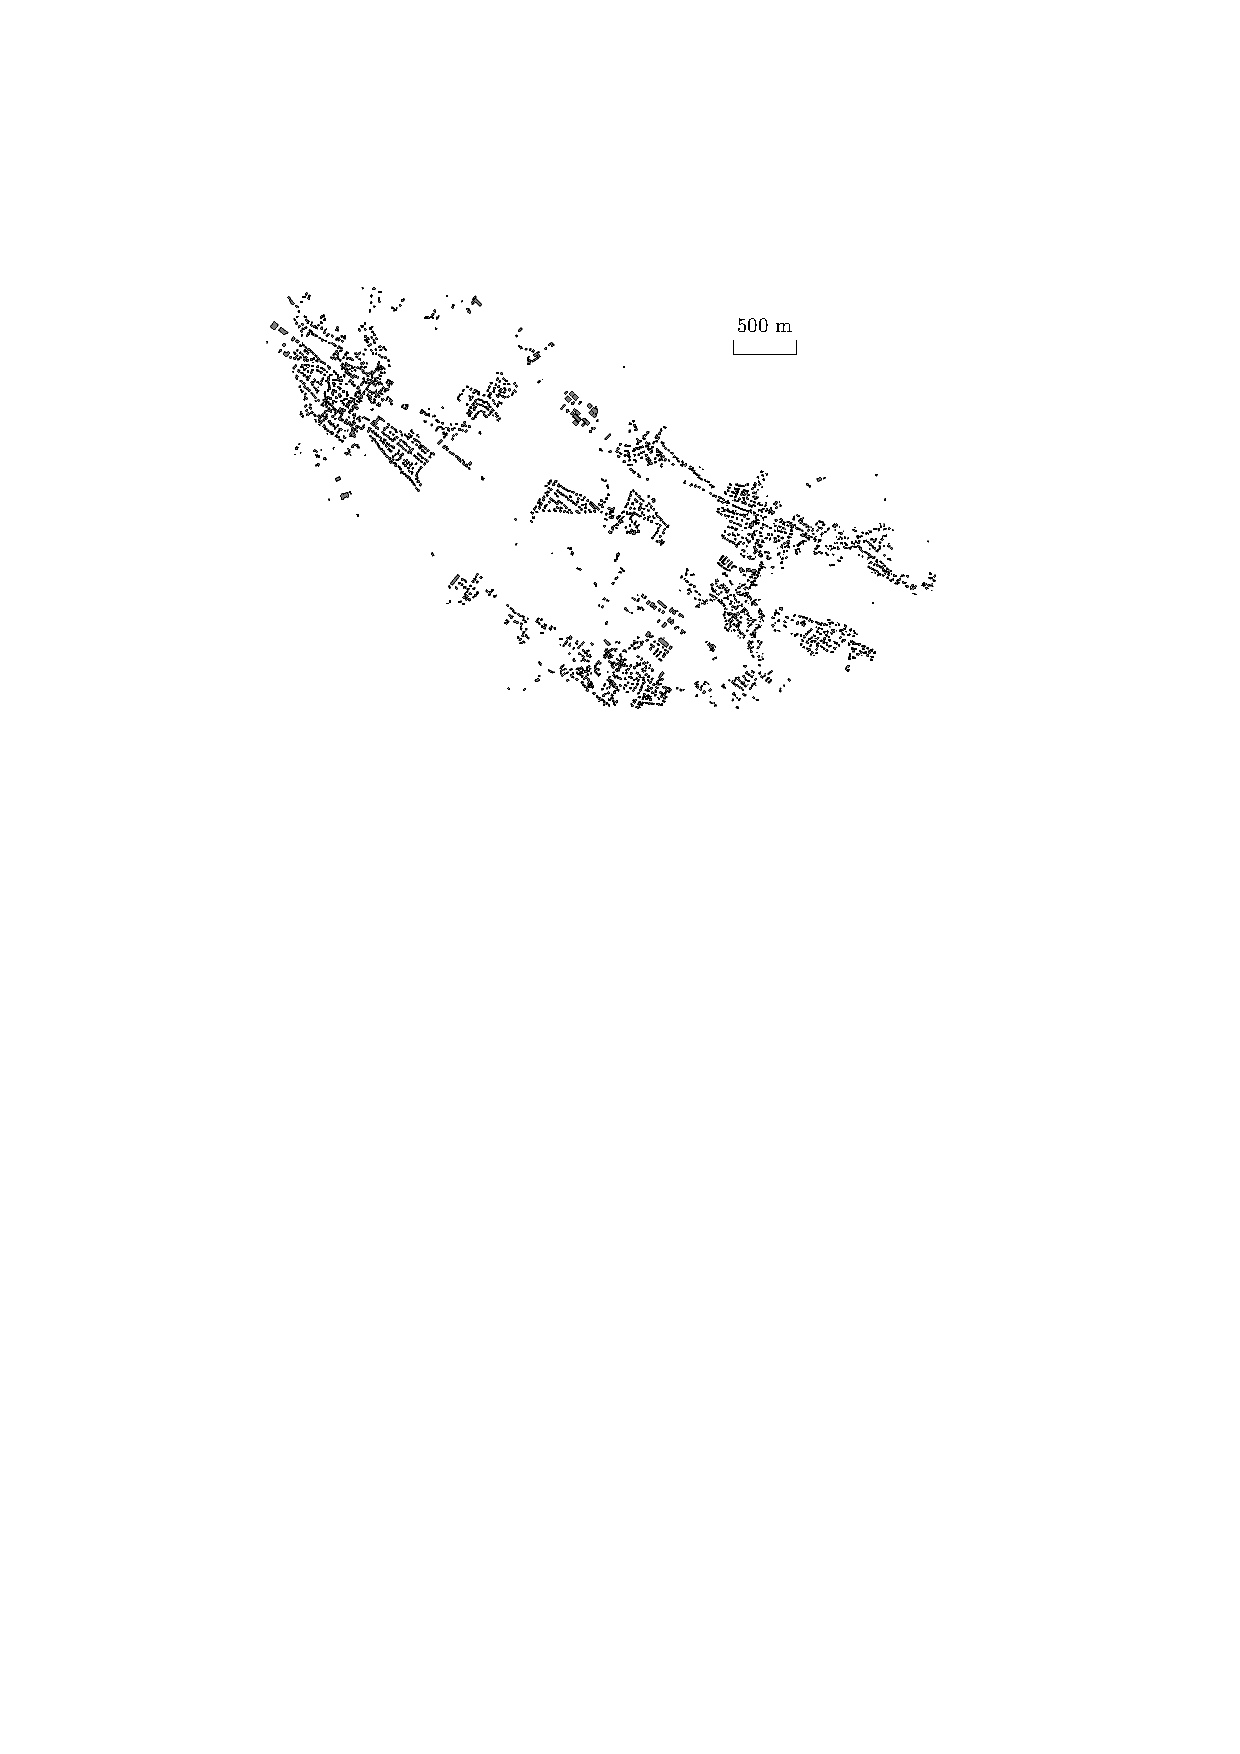
\includegraphics{Data}
	\caption{scale.}
	\label{fig:Data}
\end{figure}

\todo[inline]{comparison of simplification between Douglas--Peucker and 
Imai--Iri}

\subsection{Text}
\label{sec:Formalizing}



\section{Conclusions}
\label{sec:Conclusions}


To make it more efficient for on line displaying, we may need 
some external memories. First, we store the data at some key 
scales so that we may start a generalization from the immediate 
larger scale; $O(n)$ space. Second, we store the target shape 
for each building; $O(n)$ space. Third, we store the aggregation 
time and the target form for the aggregated shape; $O(n^2)$ 
space if we count vertex number.
%
The displaying time is dependent on buffering and clipping.


We our intermediate results may violate more cartographic rules, but we try to 
make the results at goal scales violate as few rules as possible.


Eventually, our result is a set of settlement boundaries. An interesting 
problem is to compare our method with \textcite{Chaudhry2008}.

We used radical law. We may also consider the fractal nature of maps proposed 
by \textcite{Jiang2015}.

We did not include streets. We can either put them above the settlement 
boundaries on map, or use them as restriction for building growing.

Show some results obtained by ArcGIS.
Show the data at $1:50{,}000$.

\todo[inline]{consider multi bridges; 
	consider transparency of bridges in stead of enlarging}

\printbibliography
\end{document}